%! Probability Models — Unit 3, Lesson 3.2 — Guided Notes & Practice
% THE in-class document, in the MAIN IDEAS / NOTES shape (LESSON_SHAPE.md §1): the vocabulary
% box, the hook, then ONE two-column guidednotes table. Problems run 1..14.
% Unit timing (5/45/5/5): I do ~25 min (rows 1-4), Guided Practice ~20. 4 pages at 12pt: a ceiling.
%   I DO   : the teacher reads the definition, marks up the display, works 1, 3, 5, 7.
%   WE DO  : the class works the rest of each grid; the Guided Practice (11-14) is worked together.
%   YOU DO : nothing on this page. ../homework/ is the individual practice.
% THE TRAP: problem 8 (whole circle read as "only": 15 for 10).
% THE CRUX: problem 9 (the hook vote re-taken: 18 + 15 = 33, but the union is 28).
% Problem 13 is the crux transferred. Scope: NO addition-rule formula (3.3), NO multiplying along
% branches (3.3), NO independence or conditional probability (3.3-3.4).
%
% THE DATA
%   Wheel, 8 equal sectors: drink 1,3,6; dessert 2,7; taco 5; try again 4,8.
%     P(drink) = 3/8 = 0.375 = 37.5%; 200 spins -> 75; P(not drink) = 5/8; P(prize) = 1 - 2/8 = 3/4.
%   Combo orders (120): Taco 60 (L 45, W 15), Burger 40 (L 25, W 15), Noodles 20 (L 10, W 10);
%     Lemonade 80, Water 40. P(burger and water) = 15/120 = 1/8; P(lemonade) = 80/120 = 2/3.
%   Festival survey (40): taco 18, lemonade 15, both 5; only taco 13, only lemonade 10;
%     union 28 (7/10); neither 12 (3/10); Dani's sum 33.
%   Roster (30): soccer 15, basketball 9, both 4; only soccer 11, only basketball 5; union 20
%     (2/3); neither 10 (1/3); the coach's sum 24.
% TABLE MECHANICS: inside a cell, `\\` ENDS THE ROW: break lines with \par. A row cannot break
% across pages: the figure gets its own sub-row and each grid row is its own sub-row.
% NO SKETCH QUESTIONS: every display is pre-drawn in TikZ (or set as a table) and read.
\documentclass[12pt]{article}
\usepackage{saar-article}
\usepackage{saar-boxes}
\newcommand{\TallMath}[1]{$\displaystyle #1\rule[-1.4em]{0pt}{3.2em}$}
% Word bank strip: ONLY above a table the student fills (row 3).
\newcommand{\wordbank}[1]{\par\vspace{2pt}\noindent\fcolorbox{goldacc}{goldbg}{\parbox{\dimexpr\linewidth-2\fboxsep-2\fboxrule\relax}{\small\textbf{Word bank:} #1}}\par\vspace{4pt}}
% Vocabulary rows: a FIXED-HEIGHT row carrying the term label and OPEN writing space. The key
% fills exactly the same height. Keep key definitions to two lines.
\newcommand{\termrowheight}{2.3cm}
\newlength{\termrowinset}\setlength{\termrowinset}{7pt}
\newcommand{\vterm}[1]{%
  \par\noindent\begin{minipage}[t][\termrowheight][t]{\linewidth}%
    \vspace*{\termrowinset}%
    \textbf{\textcolor{cerulean}{#1:}}%
  \end{minipage}\par}
\newcommand{\vtermans}[2]{%
  \par\noindent\begin{minipage}[t][\termrowheight][t]{\linewidth}%
    \vspace*{\termrowinset}%
    \textbf{\textcolor{cerulean}{#1:}}\quad\ans{#2}%
  \end{minipage}\par}
% The prize wheel: #1 radius (cm), #2 the eight sector/fill pairs, #3 the label for each sector
% is drawn by \wheellabel, set just before the call.
\newcommand{\sectorwheel}[2]{%
  \begin{tikzpicture}
    \foreach \i/\c/\t in {#2} {
      \fill[\c] (0,0) -- ({90-45*(\i-1)}:#1) arc[start angle={90-45*(\i-1)}, end angle={90-45*\i}, radius=#1] -- cycle;
    }
    \foreach \i/\c/\t in {#2} {
      \draw[thick, charcoal] (0,0) -- ({90-45*(\i-1)}:#1);
      \node[align=center, font=\scriptsize, inner sep=0pt] at ({90-45*(\i-0.5)}:{0.68*#1}) {\t};
    }
    \draw[thick, charcoal] (0,0) circle[radius=#1];
    \fill[redacc] (0,{#1+0.05}) -- (-0.14,{#1+0.32}) -- (0.14,{#1+0.32}) -- cycle;
  \end{tikzpicture}}
% One Venn diagram frame: #1 left-circle title, #2 right-circle title, then the four regions
% (only left, both, only right, neither), then the group's label.
\newcommand{\vennframe}[7]{%
  \begin{tikzpicture}
    \draw[thick, charcoal, fill=white] (-4.25,-1.8) rectangle (4.25,2.0);
    \begin{scope}[blend mode=multiply]
      \fill[frost] (-1.05,0) circle[radius=1.55];
      \fill[goldbg] (1.05,0) circle[radius=1.55];
    \end{scope}
    \draw[thick, cerulean] (-1.05,0) circle[radius=1.55];
    \draw[thick, goldacc] (1.05,0) circle[radius=1.55];
    \node[font=\footnotesize\bfseries, align=center] at (-3.1,1.5) {#1};
    \node[font=\footnotesize\bfseries, align=center] at (3.1,1.5) {#2};
    \node at (-1.6,0) {#3};
    \node at (0,0) {#4};
    \node at (1.6,0) {#5};
    \node at (3.45,-1.3) {#6};
    \node[font=\scriptsize\itshape, anchor=north] at (0,1.98) {#7};
  \end{tikzpicture}}

\begin{document}

\pageheader{Unit 3, Lesson 3.2}{Guided Notes \& Practice}
% NAMESTRIP: no \namedateperiod here. The student writes their name once, on the
% cover this component is stapled behind.

\vspace{0.15in}

\boxguard[16]
\begin{vocabbox}
\small
Fill in each term \textbf{as we name it} in the notes below.
\vterm{Sample space}
\vterm{Event}
\vterm{Complement}
\vterm{Mutually exclusive}
\end{vocabbox}

\boxguard[12]
\begin{hookbox}
\small
A food-truck festival surveyed $40$ students. $18$ bought a taco and $15$ bought a lemonade; a
student could buy one, both, or neither. Dani adds: \emph{``$18 + 15 = 33$, so $33$ of the $40$
bought a taco or a lemonade.''}

\vspace{3pt}
\textbf{Is Dani's count right?} Circle one: \quad right \qquad too high \qquad too low \qquad
can't tell yet --- and say why. We vote again at problem~9.
\par\writelines{2}
\end{hookbox}

\small
\begin{guidednotes}
% ── ROW 1: sample space, event, theoretical probability, expected count ──────
\mainidea[Outcomes and predictions]{Theoretical Probability} &
The \textbf{sample space} is the set of all possible outcomes; an \textbf{event} is any set of
those outcomes. When the outcomes are equally likely, $P(\text{event}) =
\dfrac{\text{outcomes in the event}}{\text{outcomes in the sample space}}$. The
\textbf{expected count} is $P(\text{event}) \times$ the number of trials: a prediction, not a promise.
\\
& {\centering
{\footnotesize\textbf{The festival's prize wheel: one spin, $8$ equal numbered sectors}}\par\vspace{3pt}
\sectorwheel{1.95}{1/frostmid/\textbf{1}\\Drink, 2/goldbg/\textbf{2}\\Dessert, 3/frostmid/\textbf{3}\\Drink, 4/graybg/\textbf{4}\\Try\\again, 5/greenbg/\textbf{5}\\Taco, 6/frostmid/\textbf{6}\\Drink, 7/goldbg/\textbf{7}\\Dessert, 8/graybg/\textbf{8}\\Try\\again}\par}
\\
& \begin{probgrid}{|Y|Y|}
\pcell{1}{Kira counts four prize names and says $P(\text{free drink}) = \frac14$. List the sample space and the event $D$ = free drink. Give the correct $P(D)$ as a fraction, a decimal, and a percent.}{2.0cm}{} & \pcell{2}{The truck expects $200$ spins on Saturday. About how many free drinks should it plan for? Why ``about''?}{2.0cm}{} \\ \hline
\end{probgrid}
\\ \hline
% ── ROW 2: complement rule; complementary vs mutually exclusive ──────────────
\mainidea[Complementary or mutually exclusive?]{Complement Rule} &
The \textbf{complement} of $A$ is everything in the sample space that is not in $A$, so
$P(\text{not } A) = 1 - P(A)$. \textbf{Mutually exclusive} events cannot both happen on one
outcome. \textbf{Complementary} events are mutually exclusive \emph{and} together cover the whole
sample space.
\\
& {\centering
\begin{minipage}[t]{0.49\linewidth}\centering
{\footnotesize\textbf{Free drink / not a free drink}}\par\vspace{2pt}
\sectorwheel{1.2}{1/frostmid/1, 2/goldbg/2, 3/frostmid/3, 4/goldbg/4, 5/goldbg/5, 6/frostmid/6, 7/goldbg/7, 8/goldbg/8}\par\vspace{3pt}
These are:\ \labelbox{3.9cm}{}
\end{minipage}\hfill
\begin{minipage}[t]{0.49\linewidth}\centering
{\footnotesize\textbf{Free drink / free dessert}}\par\vspace{2pt}
\sectorwheel{1.2}{1/frostmid/1, 2/goldbg/2, 3/frostmid/3, 4/white/4, 5/white/5, 6/frostmid/6, 7/goldbg/7, 8/white/8}\par\vspace{3pt}
These are:\ \labelbox{3.9cm}{}
\end{minipage}\par}
\\
& \begin{probgrid}{|Y|Y|}
\pcell{3}{Use the complement rule to find $P(\text{not a free drink})$ and $P(\text{win a prize})$. (A prize is the complement of ``try again.'')}{2.2cm}{} & \pcell{4}{Complementary, mutually exclusive only, or neither? How do you know? \par (a) free drink; free dessert \par (b) free drink; even-numbered sector}{2.2cm}{} \\ \hline
\end{probgrid}
\\ \hline
% ── ROW 3: one situation as a tree and a two-way table ───────────────────────
\mainidea[One situation, two organizers]{Tree and Two-Way Table} &
A \textbf{tree diagram} follows one choice, then the next, along branches. A \textbf{two-way
table} crosses the same two choices as rows and columns. The tree's branch ends are the table's inside cells.
\\
& {\footnotesize\textbf{The Combo Truck's $120$ orders: a meal, then a drink. Fill the table from the tree.}}\par\vspace{3pt}
\begin{minipage}[c]{0.47\linewidth}\centering
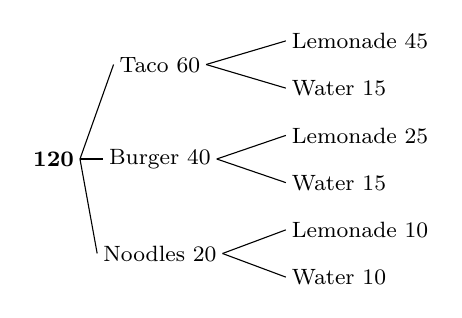
\begin{tikzpicture}[x=1cm, y=0.6cm, font=\footnotesize, inner sep=2pt]
  \node (r) at (0,0) {\textbf{120}};
  \node (a) at (1.35,2)  {Taco $60$};
  \node (b) at (1.35,0)  {Burger $40$};
  \node (c) at (1.35,-2) {Noodles $20$};
  \draw (r.east) -- (a.west); \draw (r.east) -- (b.west); \draw (r.east) -- (c.west);
  \node[anchor=west] (a1) at (2.95,2.5)  {Lemonade $45$};
  \node[anchor=west] (a2) at (2.95,1.5)  {Water $15$};
  \node[anchor=west] (b1) at (2.95,0.5)  {Lemonade $25$};
  \node[anchor=west] (b2) at (2.95,-0.5) {Water $15$};
  \node[anchor=west] (c1) at (2.95,-1.5) {Lemonade $10$};
  \node[anchor=west] (c2) at (2.95,-2.5) {Water $10$};
  \draw (a.east) -- (a1.west); \draw (a.east) -- (a2.west);
  \draw (b.east) -- (b1.west); \draw (b.east) -- (b2.west);
  \draw (c.east) -- (c1.west); \draw (c.east) -- (c2.west);
\end{tikzpicture}
\end{minipage}\hfill
\begin{minipage}[c]{0.5\linewidth}\centering
{\renewcommand{\arraystretch}{1.5}%
\begin{tabular}{@{}l c c c@{}}
\toprule
& \textbf{Lem.} & \textbf{Water} & \textbf{Total} \\
\midrule
Taco & \blank{1.0cm} & \blank{1.0cm} & 60 \\
Burger & \blank{1.0cm} & \blank{1.0cm} & 40 \\
Noodles & \blank{1.0cm} & \blank{1.0cm} & 20 \\
\textbf{Total} & \blank{1.0cm} & \blank{1.0cm} & 120 \\
\bottomrule
\end{tabular}}
\end{minipage}
\\
& \begin{probgrid}{|Y|Y|}
\pcell{5}{One order is picked at random. Find $P(\text{burger and water})$. Which path on the tree shows it?}{2.0cm}{} & \pcell{6}{Find $P(\text{lemonade})$. Why is the table faster than the tree for this one?}{2.0cm}{} \\ \hline
\end{probgrid}
\\ \hline
% ── ROW 4: THE CRUX — Venn diagram ───────────────────────────────────────────
\mainidea[Every region once]{Venn Diagram} &
A \textbf{Venn diagram} sorts one group by two events. The overlap is the \textbf{intersection}
($A$ \emph{and} $B$). Everything inside either circle is the \textbf{union} ($A$ \emph{or} $B$).
\textbf{Only} $A$ is $A$'s circle without the overlap. \textbf{Neither} is outside both circles.
\\
& {\centering\begin{minipage}[c]{0.7\linewidth}\centering
\vennframe{Taco\\($18$ in all)}{Lemonade\\($15$ in all)}{\large $13$}{\large $5$}{\large $10$}{\large $12$}{$40$ students surveyed}\end{minipage}\hfill\begin{minipage}[c]{0.28\linewidth}\centering
The $5$ is the\par\labelbox{2.6cm}{}\par\vspace{6pt}
$13 + 5 + 10$ is the\par\labelbox{2.6cm}{}\end{minipage}\par}
\\
& \begin{probgrid}{|Y|Y|}
\pcell{7}{One surveyed student is picked at random. Find $P(\text{taco and lemonade})$ and $P(\text{neither})$.}{2.0cm}{} & \pcell{8}{Reese says $P(\text{only lemonade}) = \frac{15}{40}$, because the lemonade circle holds $15$. What did Reese read? Find the correct probability.}{2.0cm}{} \\ \hline
\end{probgrid}
\\
& \begin{probgrid}{|Y|Y|}
\pcell{9}{\textbf{Vote again:} right \; too high \; too low. Dani's $18 + 15 = 33$. Count ``taco or lemonade'' region by region. Find $P(\text{taco or lemonade})$.}{2.1cm}{} & \pcell{10}{Which students did Dani count twice? Check your answer to 9 with the complement of ``neither.''}{2.1cm}{} \\ \hline
\end{probgrid}
\\
& \fcolorbox{cerulean}{frost}{\parbox{\dimexpr\linewidth-2\fboxsep-2\fboxrule\relax}{\centering
\textbf{Adding the two circle totals counts the overlap twice. To count ``or,'' add the regions inside the circles, each one once.}}}
\\ \hline
% ── ROW 5: GUIDED PRACTICE — a fresh context ─────────────────────────────────
\mainidea[Guided practice]{The Team Roster} &
A roster of $30$ athletes: $15$ play soccer, $9$ play basketball, and $4$ play both.
\\
& {\centering
\vennframe{Soccer\\($15$ in all)}{Basketball\\($9$ in all)}{\labelbox{0.9cm}{}}{\labelbox{0.9cm}{}}{\labelbox{0.9cm}{}}{\labelbox{0.9cm}{}}{$30$ athletes on the roster}\par}
\\
& \begin{probgrid}{|Y|Y|}
\pcell{11}{Fill in the four regions. Show how you found each ``only'' number and ``neither.''}{2.0cm}{} & \pcell{12}{One athlete is picked at random. Find $P(\text{only basketball})$ and $P(\text{neither sport})$.}{2.0cm}{} \\ \hline
\end{probgrid}
\\
& \begin{probgrid}*{|Y|Y|}
\pcell{13}{Coach says $15 + 9 = 24$ athletes play soccer or basketball. Find $P(\text{soccer or basketball})$. Is Coach right? Why or why not?}{2.1cm}{} & \pcell{14}{Are ``soccer'' and ``basketball'' mutually exclusive? Are ``soccer or basketball'' and ``neither'' complementary? How does the diagram show it?}{2.1cm}{} \\ \hline
\end{probgrid}
\\ \hline
\end{guidednotes}

% ── THE NOTES END AT GUIDED PRACTICE ─────────────────────────────────────────
% There is deliberately no "you do" here: ../homework/ is the individual practice.

\end{document}
